% !TEX encoding = UTF-8
% !TEX TS-program = pdflatex
% !TEX root = ../tesi.tex
% !TEX spellcheck = it-IT

%**************************************************************
\chapter{Valutazione Retrospettiva}
\label{cap:valutazione-retrospettiva}
%**************************************************************
\intro{Questo capitolo riporta un bilancio finale su quanto svolto durante lo stage.}




%**************************************************************************************************
\section{Bilancio sui risultati}
In questa sezione riassumo gli obiettivi aziendali e gli obiettivi personali raggiunti durante lo stage.
\subsection{Obiettivi conseguiti}
Gli obiettivi fissati all'inizio dello stage hanno subito delle modifiche perché l'azienda ha voluto privilegiare il porting di DRE. Il \emph{porting} dell'applicativo è parzialmente completato, l'unica funzionalità non ancora implementata una procedura di \emph{map-reduce}. Quest'ultima funzionalità non l'ho completata perché implementata con la tecnologia javascript da eseguire all'interno di MongoDb, le mie competenze per comprendere quel codice erano insufficienti ed avrebbero introdotto un ulteriore ritardo per lo sviluppo di Tres inoltre l'obiettivo di migliorare la fase di apprendimento di questo modulo non l'ho raggiunto. Durante lo sviluppo di Tres ho individuato 23 requisiti di cui 20 obbligatori e 3 desiderabili.  
\begin{figure}[h]
\centering
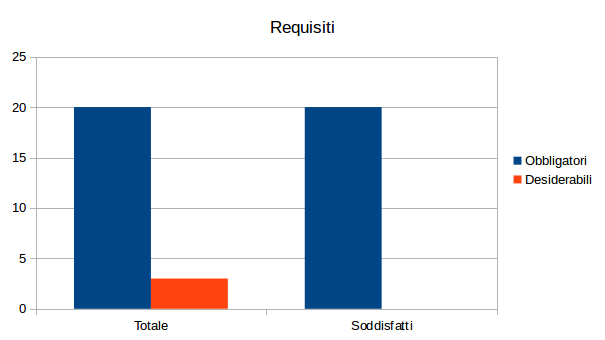
\includegraphics[scale=0.62]{immagini/graficorequisiti}
\caption{Riassunto requisiti}
\label{fig:client-server}
\end{figure}
\\I requisiti non soddisfatti riguardano direttamente gli obiettivi (e quindi non ho raggiunto) di implementazione di algoritmi di \emph{clustering} e di implementazione di algoritmi per l'individuazione dei gusti dell'utente. Tuttavia quest'ultimo obbiettivo l'ho centrato grazie all'implementazione di ID3 per fornire una raccomandazione sulla base del comportamento utente. Infine in questa attività ho soddisfatto l'obbiettivo minimo riguardante l'utilizzo di OrientDb.
\subsection{Obiettivi personali}
All'inizio dello stage il mio obbiettivo era quello di imparare nuove tecnologie da aggiungere alle mie conoscenze perché ritenevo il mio bagaglio personale insufficiente per affrontare il mondo del lavoro. Questo obbiettivo è stato certamente raggiunto, infatti lo stage mi ha permesso di padroneggiare ad un buon livello tecnologie quali OrientDb, web framework di concezione moderna e Scala. Quest'ultimo mi ha dato la possibilità di apprendere le nozioni per un corretto stile di programmazione funzionale, che era uno degli obbiettivi prefissatomi. Ritengo l'obbiettivo riguardante l'approfondimento di argomenti quali, intelligenza artificiale e i sistemi di raccomandazione, parzialmente soddisfatto. Durante lo stage non ho trovato il supporto necessario per approfondire queste competenze, soprattutto per quanto riguarda i sistemi di raccomandazione visto la natura del progetto di stage.
%**************************************************************************************************




%**************************************************************************************************
\section{Bilancio formativo}
In questa sezione viene riportato le competenze acquisite durante lo stage.
%**************************************************************************************************




%**************************************************************************************************
\section{Distanza tra formazione universitaria e lavoro}
In questa sezione sezione viene esposto la valutazione personale della distanza tra la formazione ricevuta durante il corso di studi e lo stage formativo.
%**************************************************************************************************